% begin module exponential-function-ex-sketch
\begin{frame}
\begin{example}
Draw the graph of the function $y = 2^{-x}-1= 0.5^x-1= \left(\frac{1}{2}\right)^x-1 $.
\begin{columns}[c]
\column{.7\textwidth}
\psset{xunit=1cm, yunit=1cm}
\begin{pspicture}(-5, -5)(5,5) 
\psframe*[linecolor=white](-5,-5)(5,5) 
\psaxes[ticks=none, labels=none]{<->}(0,0)(-4, -2.5)(4,4)
\psline(-0.1,1)(0.1, 1)
\rput[l](0.2, 1){$1$} 
\psline(1,0.1)(1, -0.1)
\rput[t](1, -0.2){$1$} 
\psline(-0.1,-1)(0.1, -1)
\rput[tl](0.2, -1){$-1$} 
%Function formula: 2^{x} 
\uncover<2>{
\psplot[linecolor=red, plotpoints=1000]{-4}{2}{2 x exp}
\rput[l](1.7, 3){$y=2^x$}
}
\uncover<3->{
\psplot[linecolor=gray, plotpoints=1000]{-4}{2}{2 x exp}
\rput[l](1.7, 3){\color{gray}$y=2^x$}
}
\uncover<3>{
\psplot[linecolor=red, plotpoints=1000]{-2}{4}{0.5 x exp}
\rput[l](-1.5, 3.2){$y=0.5^x$}
}
\uncover<4->{
\psplot[linecolor=gray, plotpoints=1000]{-2}{4}{0.5 x exp}
\rput[l](-1.5, 3.2){\color{gray}$y=0.5^x$}
}
\uncover<4->{
\psplot[linecolor=red, plotpoints=1000]{-2.321928095}{4}{0.5 x exp -1 add}
\rput[r](-1.7, 2){$y=0.5^x-1$}
\psline[linecolor=blue, linestyle=dashed](-4, -1)(4, -1)
}
\end{pspicture}
%\only<handout:0| -1>{%
%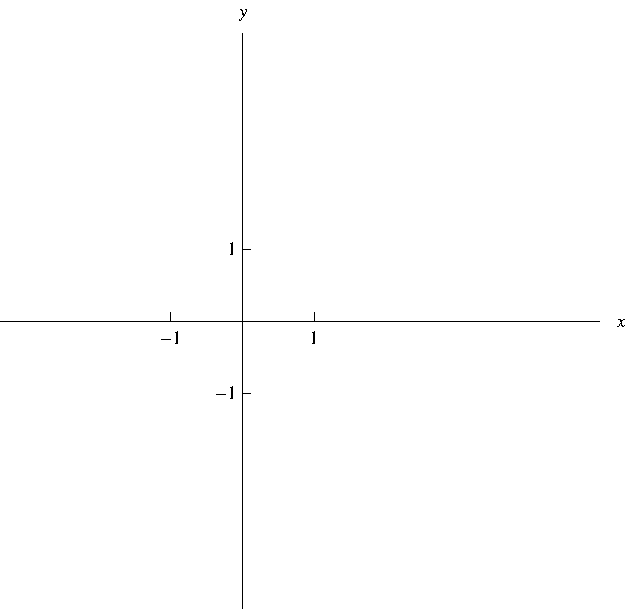
\includegraphics[height=7cm]{exponential-functions/pictures/07-02-ex1a.pdf}%
%}%
%\only<handout:0| 2>{%
%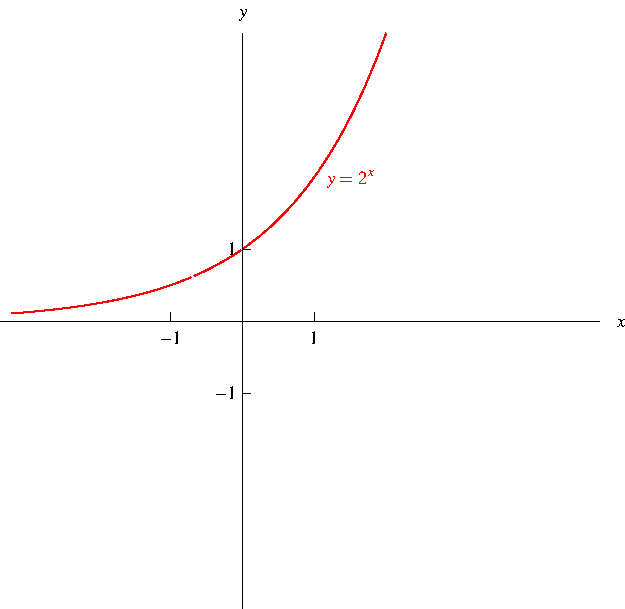
\includegraphics[height=7cm]{exponential-functions/pictures/07-02-ex1b.pdf}%
%}%
%\only<handout:0| 3>{%
%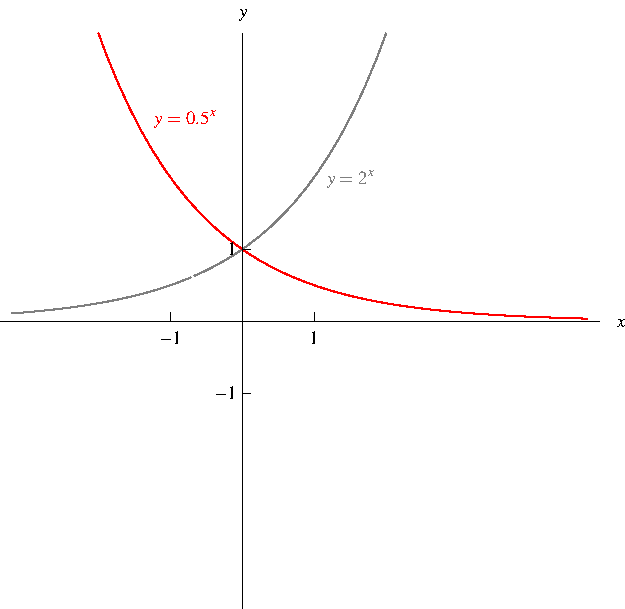
\includegraphics[height=7cm]{exponential-functions/pictures/07-02-ex1c.pdf}%
%}%
%\only<4->{%
%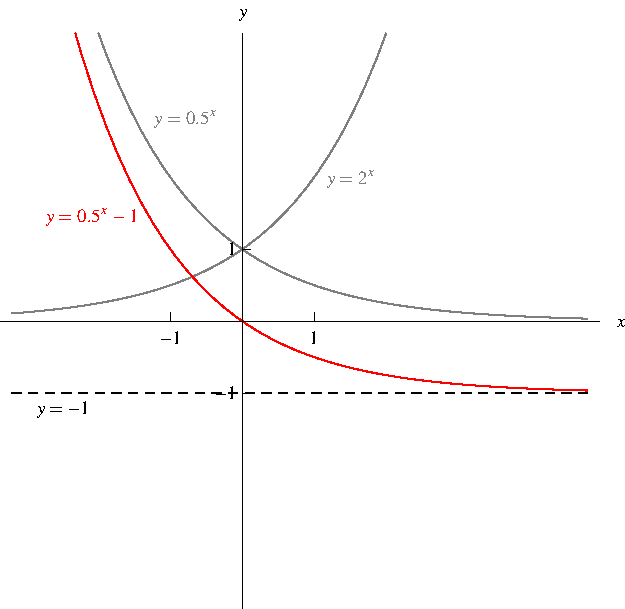
\includegraphics[height=7cm]{exponential-functions/pictures/07-02-ex1d.pdf}%
%}%
\column{.3\textwidth}
Recall from previous lectures.
\begin{itemize}
\item<2-> Plot of $2^x$ assumed given.
\item<3-> Plot $f(-x)$ = reflect $f(x)$ across $y$ axis.
\item<4-> Plot $g(x)-1$ = shift graph $g(x)$ 1 unit down.
\end{itemize}
\end{columns}
\end{example}
\end{frame}
% end module exponential-function-ex-sketch